% % ------------------------------------------------------------------------------

% % ------------------------------------------------------------------------------
% \documentclass[12pt]{report} 

% %\usepackage{projectreport}

% % Preamble
% \usepackage{graphicx}
% \usepackage{setspace}
% \usepackage[table,xcdraw]{xcolor}
% \usepackage[a4paper, margin=1in]{geometry}
% \usepackage{appendix}
% \usepackage[superscript]{cite}
% \usepackage{float}
% \usepackage{listings}
% \usepackage{color}
% \usepackage{hyperref}
% \usepackage{adjustbox}
% \usepackage{caption}
% \usepackage{setspace}
% \usepackage{soul}
% \usepackage{multirow}
% \usepackage{tikz}
% \usepackage{modiagram}
% \usepackage{chemscheme}
% \usepackage{chemfig}
% \usepackage[version=4]{mhchem}
% \usepackage{enumitem}
% \usepackage{pdflscape}
% \usepackage{gensymb}
% \bibliographystyle{unsrt}

% % % Word count (requires --shell-escape)
% % \newcommand{\wordcount}{%
% %   \immediate\write18{texcount -1 -sum -merge -q main.tex > main-wordcount.sum}%
% %   \input{main-wordcount.sum}%
% % }
 


% % ------------------------------------------------------------------------------
% % Enter your details here
% % ------------------------------------------------------------------------------
% \newcommand{\name}{Thomas P. Dean}
% \newcommand{\studentno}{201494370}
% \newcommand{\course}{MNatSc. Master of Natural Sciences }
% % \newcommand{\course}{BSc. Computer Science}
% % \newcommand{\course}{MEng. Computer Science}
% \newcommand{\projecttitle}{An Investigation into a Self-Healing Polyimide Towards Soft Robotic Implications }
% \newcommand{\submissiondate}{October 2025}
% \newcommand{\submissionyear}{2025}

% % ------------------------------------------------------------------------------
% % Document
% % ------------------------------------------------------------------------------
% \begin{document}

% \maketitle
% % ------------------------------------------------------------------------------
% % Top matter
% % ------------------------------------------------------------------------------
% % \chapter*{Abstract}
% % \blindtext[1] % creates dummy text

% % \chapter*{Intellectual Property}
% % The candidate confirms that the work submitted is his/her own and that appropriate credit has been given where reference has been made to the work of others.

% % This copy has been supplied on the understanding that it is copyright material and that no quotation from the thesis may be published without proper acknowledgement.

% % © \submissionyear\ The University of Leeds, \name

% % \vspace{2cm}
% % Signed 
% % \makebox[4cm][c]{\raisebox{-2ex}{\includegraphics[width=3cm, height=1cm]{example-image}}} % replace with your signature

% % \chapter*{Acknowledgements}
% % This research has been carried out by a team which has included (name the individuals). My own contributions, fully and explicitly indicated in the thesis, have been......(please specify)” The other members of the group and their contributions have been as follows: (please specify).

% \chapter*{Abstract}
%  
Continuum robots are a type of soft robot heavily inspired by the motion of elephant trunks. They are able to navigate complex environments through their innate actuation methods and material properties. To achieve fully soft devices, pneumatic actuators are often used, however, the materials used in these actuators are typically delicate and are prone to failure. Recently, an approach to mitigate this is the use of self-healing polymers. This report covers the investigation of a new material based on a polyimide to achieve self-healing capabilities and its use in a soft continuum robot.



% %\noindent\textbf{Word count: \wordcount}


% \tableofcontents
% \listoffigures
% % \listoftables

% % ------------------------------------------------------------------------------
% % Main matter
% % Chapters are added to the document using the \include{chapterx} command
% % ------------------------------------------------------------------------------
% \newpage
% \setcounter{page}{0}
% \pagenumbering{arabic}
% % ------------------------------------------------------------------------------
% Chapter 1
% Delete this content and replace with your own
%tis is a test sentence
% ------------------------------------------------------------------------------
\chapter{Introduction} % enter the name of the chapter here
\label{cha:introl} % enter the chapter label here (for cross referencing)

% \input{background}

\begin{figure}
    \centering
    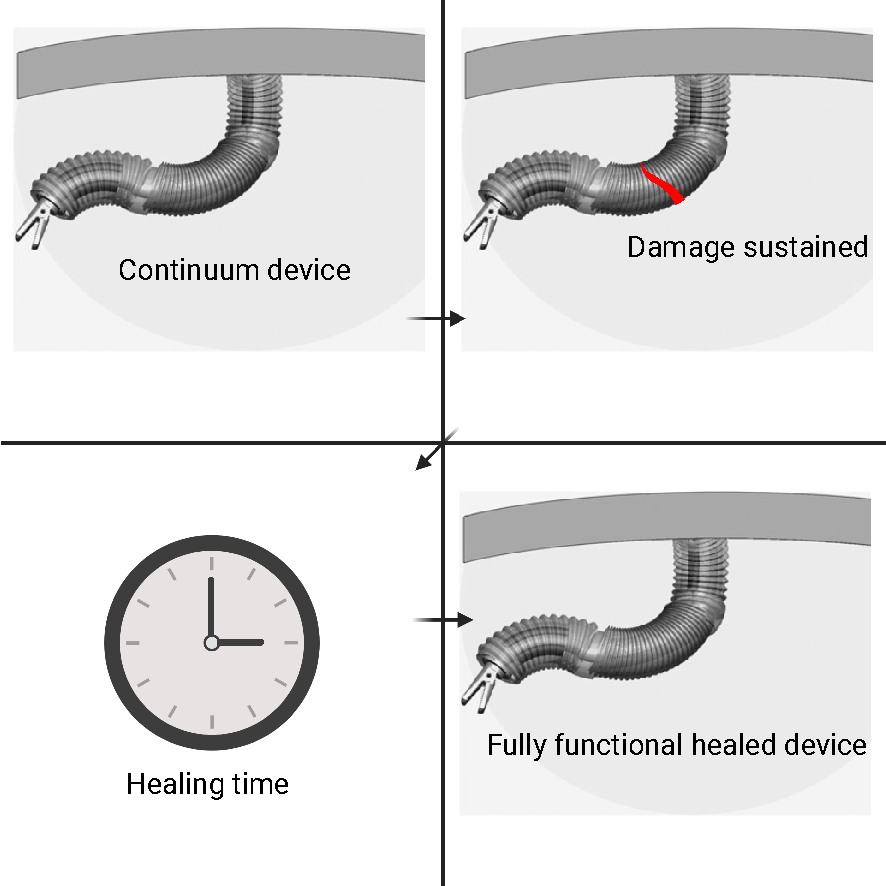
\includegraphics[width=0.8\linewidth]{Images/overview v3.pdf}
    \caption{A continuum device sustaining damage before self-healing and regaining full functionality using a modified image from \cite{cianchetti2014soft}}
    \label{fig:overview}
\end{figure}

\section{Importance and Applications of Soft Robotics}
Soft robots are devices known for their use of soft materials, compliant nature and near infinite degrees of freedom. Degrees of freedom (DOF) is a term related to the number of independent movements a robot can make in 3D space \cite{lynch2017modern}. Soft robots are usually nature inspired such as ``vine-like'' tip growing robots \cite{hawkes2017soft, davy2025magnetic}, ``snake like'' continuum robots \cite{anderson1967tenser, lloyd2020learnt} and ``hand-like'' soft grippers \cite{ilievski2011soft, guo2018soft}. The advantages of using a body that is highly deformable and with near-infinite DOF means these devices can be actively controlled to navigate tortuous environments with ease. 

This report focuses on continuum robots, often characterised by their long flexible bodies, commonly used for navigation and delivery or retrieval of objects in constrained environments \cite{russo2023continuum}. Continuum robots can be classified into ``continuous backbone'' and ``segmented back-bone'' designs \cite{russo2023continuum}. Continuous backbone devices are made from a soft and compliant material, in this report we will call these ``soft-bodied'', whereas, a segmented backbone refers to those that are made from hard, inflexible segments that are flexibly attached to achieve high curvatures, referred to here as ``hard-bodied''.

Hard-bodied continuum robots benefit from stiffer materials allowing a greater ease of control \cite{russo2023continuum} which can improve dexterity. However, they do not easily deform and are therefore more likely to impart a greater force on the surrounding environment \cite{davy2024vine}.  Hard continuum robots are often tendon driven, whereby the segments are joined by wires that can be pulled to give specific movements. Whereas soft bodied continuum robots can achieve high curvatures and low forces on surroundings \cite{rus2015design}, but are often harder to control due to their methods of actuation \cite{russo2023continuum} and can suffer from material failure \cite{abidi2017intrinsic}. Soft continuum robots commonly take the form of an inflated body, these can be controlled in many ways such as varying pressure \cite{hawkes2017soft}, strain limiting a specific region \cite{guo2024encoded, dean2025anisotropic} or magnetic actuation \cite{davy2025magnetic, davy2024vine}. Pressurised systems that rely on fluids need a constant seal to maintain function as opposed to a segmented tendon driven approach that can be partially damaged and remain actuatable. This motivates the utilisation of resilient materials, such as self-healing polymers, for soft robotic contexts.



\section{Types of Self-Healing Polymers}

\begin{figure}
    \centering
    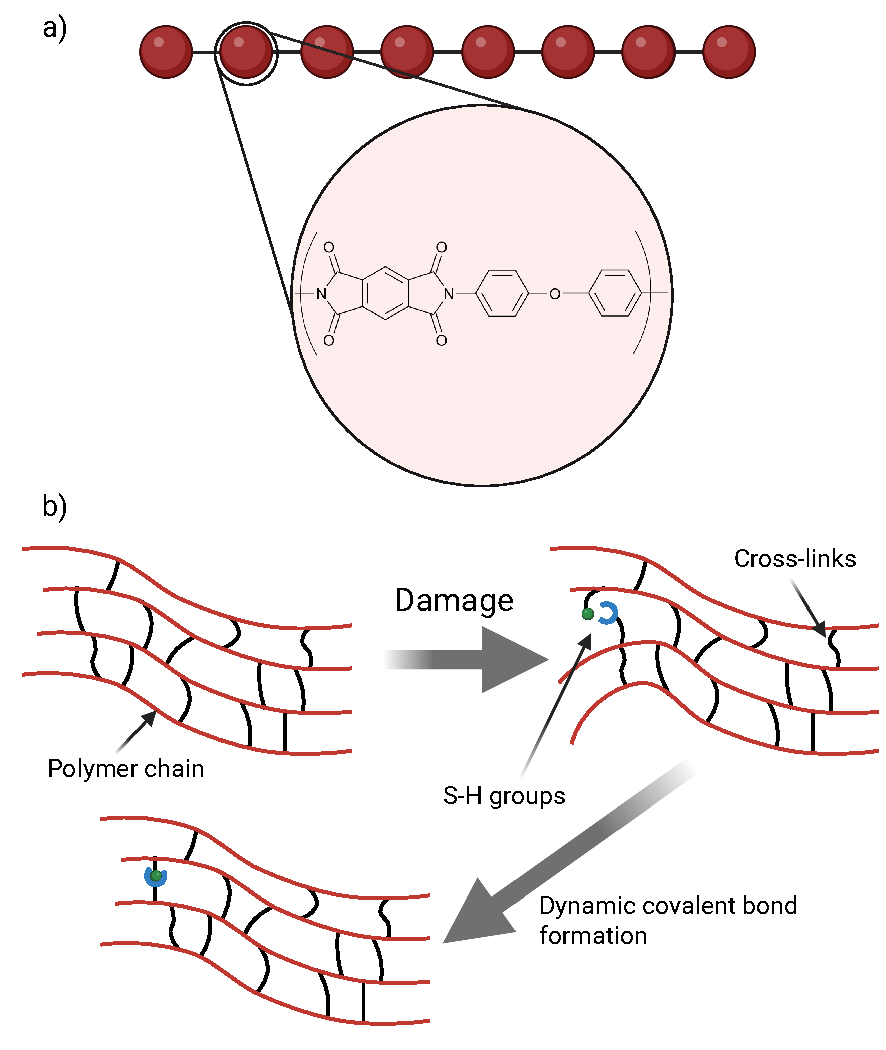
\includegraphics[width=1\linewidth]{Images/Self healing polymer.pdf}
    \caption{a) The polymer chain with a repeating chemical sub-unit. b) The mechanism of damage and repair for a self-healing polymer}
    \label{fig:shpolymer}
\end{figure}

Polymers are a type of molecule that consists of several repeating sub-units, these form chains that are combined many times over to form materials. Self-healing (S-H) polymers are a type of polymer that can heal damage \cite{srivastav2025comprehensive}. This occurs through reactions and interactions between multiple polymer chains to reconnect chains that have been shifted apart through damage. The process of damaging or cutting a polymer does not break bonds in the polymer backbone but instead can break interchain interactions called cross-linking, allowing the chains to drift apart, reforming the cross-linking interactions will ``heal" the material \cite{binder2013self}. 

S-H polymers can be classified into intrinsic or extrinsic healing, and autonomous or non-autonomous \cite{terryn2021review}. Materials with an intrinsic healing capacity involve a healing mechanism through chemical bonds or interactions that are continuously present in the polymer, rather than extrinsic healing, such as capsules of ``healing" material that are broken through damage and causing the material to reform \cite{white2001autonomic}. Autonomy refers to the healing process occurring without external input. For example, capsules that burst upon damage of the material and release a healing agent are classified as autonomous, whereas a photochemical reaction that needs UV light to activate \cite{trenor2004coumarins,froimowicz2011photoreactive} is a non-autonomous mechanism. 


\section{Comparison of Different Self-Healing Pathways}
There are a variety of different pathways that can be taken to create a S-H polymer depending on the chemistry of the initial polymer. The pathways that will be focused on are intrinsically self-healed types, however, both autonomous and non-autonomous types will be considered.

The three pathways below rely on a property of some electrons called conjugation. Conjugation occurs when specific electron orbitals overlap in such as way that allows the electrons to move around the molecule. This is often exploited with a property of some atoms called electronegativity, having a highly electronegative atom in a molecule will attract conjugated electrons to create a local high density region of electrons and therefore a polarisation in a molecule. 

Dynamic covalent bonds can form and break based on the conditions applied to them \cite{guo2025diels} and they are ideal for use as mechanisms for S-H due to their intrinsic nature and reliability in production of high yields \cite{nicolaou2002diels}. This report investigates the use of two types of dynamic covalent bonding, Diels-Alder and Michael additions, and an example of a supramolecular interaction. Supramolecular chemistry is based on interactions that are non-covalent and may be more suited to a soft material \cite{yang2018self}. This is due to the self-healing mechanism of the cross-links that forms interactions therefore the polymer chains can move semi-independently \cite{wanasinghe2022dynamic,yang2018self}. Whereas, a dynamic covalent bond has a much higher bond energy \cite{guo2025diels} and can therefore get closer to the original physical properties of a polymer.

\subsection{Using a Diels-Alder Addition as a Self-Healing Pathway}

\begin{figure}
    \centering
    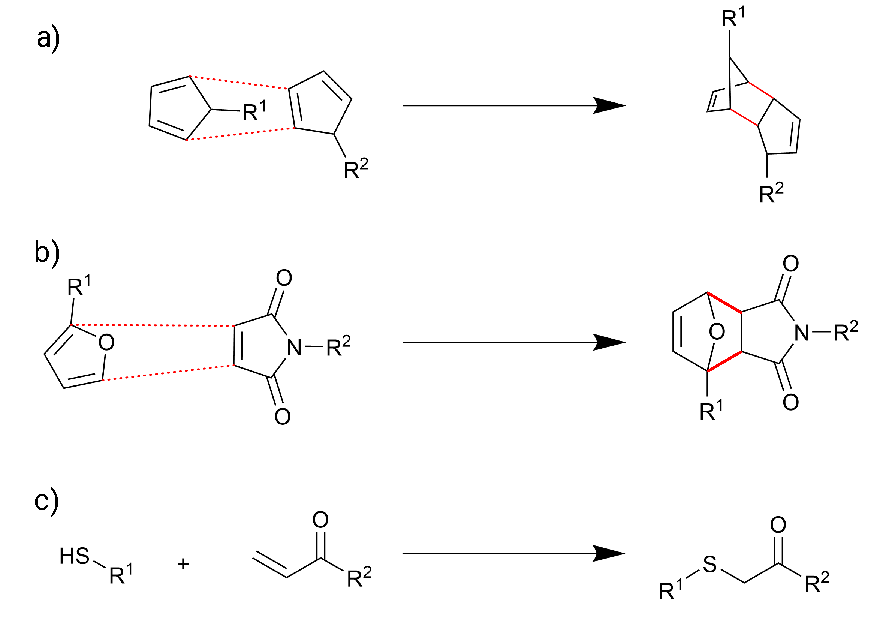
\includegraphics[width=0.8\linewidth]{Images/DA reactions.pdf}
    \caption{a) A Diels-Alder reaction between two molecules of cylopentadiene. b) A Diels-Alder reaction between a furan and maleimide. c) A Thiol-Michael Addition between a thiol and a conjugated alkene. }
    \label{fig:dareactions}
\end{figure}
Diels-Alder (DA) reactions require a diene, a class of molecule characterised by having two sets of double bonds, and an alkene (``dieneophile") \cite{ratwani2023self,guo2025diels}. The reaction occurs when conjugated electrons from the diene are free to move to form new bonds with the carbons either side of the alkene double bond, this creates a new ring structure. A faster reaction is generally observed with an electron rich diene and an electron poor dienophile \cite{briou2021trends}. The electronic character of the reagents can be altered by changing their local substituents. This class of reactions can have lots of different conditions depending on the molecules involved. Some variations can occur at room temperature \cite{huertas2009solvent}, which may make them an ideal choice for an autonomously healed medical device as the healing can occur whilst deployed in the body. However, many DA reactions are light \cite{trenor2004coumarins,froimowicz2011photoreactive} or heat activated \cite{li2014situ}.

Some molecules such as cyclopentadiene can perform a DA reaction with itself, this has the potential to be an ideal choice for a S-H polymer as the molecule will never be in close proximity to a molecule that it cannot react with. However, some evidence has shown that the bonds formed are not very strong and therefore high tensile strength materials may not be possible \cite{ratwani2023self}.

One of the most common types of DA reaction is a heat activated reaction between a derivative of both furan and maleimide \cite{ingoglia2014microencapsulation}. They react extremely accurately and require mild conditions \cite{ratwani2023self}, therefore they are very suitable for application as a robotics material.
One of the reasons that this reaction is so effective is that the maleimide has electron withdrawing carbonyl groups which make the dieneophile electron poor and therefore reacting faster. However, this mechanism has a disadvantage compared to cyclopentadiene as there are two halves of the end product. Therefore, there must be two different processes occurring to create both the furan substituted and maleimide substituted chains. This increases the number of total steps in the reaction which increases the risk of low reaction yields and wasted material. 


\subsection{Using a Thiol-Michael Addition as a Self-Healing Pathway}
Thiol Michael additions are a type of reaction that relies on a thiol, a molecule characterised by a sulfur containing group and a conjugated alkene \cite{nair2014thiol}. The conjugated alkene used in a Michael addition is with a carbonyl group that will attract the electrons from the alkene to allow the thiol group to react. This has a similar advantage to the Diels-Alder reaction that it is not totally dependant on specific reactants merely groups of reactants. Therefore slight changes can be made to the adjoining groups to tweak the reaction conditions. This has been previously shown to have been successful with a heat activated reaction that could heal scratches after 15 to 30 minutes at 60 \degree C \cite{kuhl2016self}. 

\subsection{Using a Pi-Stacking Approach as a Self-Healing Pathway}
Pi-Stacking is a type of intermolecular interaction whereby conjugated systems interact based on the neighbouring substituents determining if a region is electron rich or poor. These electron disparities cause an electrostatic interaction. This method commonly uses pyrenyl groups, these are polycyclic aromatic compounds, a very pi-electron rich species. These can be interacted with a napthalene diimide complex, an electron poor pi-system to give four pi-stacking interactions. A method has shown the creation of a polymer chain end group which can sandwich a napthalene group within two pyrenyl groups. \cite{burattini2011supramolecular}. This method can be combined with other intermolecular interactions like hydrogen bonding \cite{yuan2025self} or mettalosupramolecular interactions to give a stronger interaction \cite{mei2016highly}.


\section{Applications of Self-Healing Polymers in Soft Robotics}

Continuing the theme of biological inspiration of soft robotics, S-H polymers can be used to extend the lifespan of components. In soft continuum robots, the goal is usually to make the robot softer than the environment surrounding it \cite{rus2015design}. This presents challenges in abrasive environments that can damage the device. It is therefore evident that a damage resilient material would be useful. Damage resilient materials can take multiple forms: Damage isolation, material elasticity, physical self healing such as low melting temperature materials and chemical self healing \cite{bilodeau2017self}.



\subsection{State of the Art Self-Healing Soft Robots}
 State-of-the-art approaches using intrinsic S-H mechanisms are commonly based on DA chemistry \cite{terryn2021review}. These have been successfully implemented in tendon-driven \cite{roels2019multi} and pneumatically controlled soft robotic devices \cite{terryn2020room, terryn2017pneumatic}. Such devices are capable of recovering from macroscopic damage, including punctures and cuts. Additionally, there are non-covalent approaches that utilize hydrogen bonding in the development of soft self-healing actuators, such as in McKibben muscle designs \cite{lopez2020autonomous}.

\subsection{Requirements for Self-Healing Polymers in Soft Robotics}
Terryn \textit{et al.} \cite{terryn2021review} states that there are 5 main criteria for a S-H polymer; macroscopic damage must be healed completely; healing can take place multiple times at the same location; there are minimal material property changes after healing; elastomeric behaviour is achieved; the reprocessing and recycling of a material is possible. Here we propose that elastomeric behaviours are non-essential and a more useful requirement would involve a timely S-H reaction.  


\section{Limitations with Current Materials for Soft Robotics}

Damage control whilst a device is active can be a challenge \cite{kashef2025toward}, this shows a need for autonomous S-H \cite{terryn2021review}. Non-autonomous S-H can be made ``functionally autonomous" through the use of stimuli responsive mechanisms, however, the current options are slow in operation \cite{kashef2025toward}. Currently recovery timescales of applied S-H polymers are around 25 hours \cite{terryn2017pneumatic, bilodeau2017self}. By altering the polymer used or S-H pathway this could be improved. There is also a lack of an easy synthesis route for many of the current polymer options \cite{bilodeau2017self}, thereby increasing the cost and reducing widespread use. Also the number of damage-repair cycles in these devices are low, such as 3 or less \cite{terryn2017pneumatic}. Most devices do not achieve all five criteria laid out in the Terryn \textit{et al.} review \cite{terryn2021review}, such as the McKibben design of A. Lopez Diaz \textit{et al.} \cite{lopez2020autonomous} only reporting a healing efficiency of 65\%.

% % ------------------------------------------------------------------------------
% Chapter 2
% ------------------------------------------------------------------------------
\chapter{Project Aims and Objectives} % enter the name of the chapter here
\label{cha:aims} % enter the chapter label here (for cross referencing)

% \input{aims}



\section{Aims and Objectives of this Project}
The aim of this project is to understand the use of a self-healing polyimide in a soft robotics context.

We hypothesise that the incorporation of a S-H polyimide into soft robotic components will enhance their lifespan.


The objectives of this project are to:
\begin{itemize}
    \item Investigate the alteration of a polyimide through a Diels-Alder pathway to achieve a self-healing polymer 
    \item Investigate the processability of the modified polymer through material tests such as melting point analysis. 
    \item Based on the processability, apply the polymer to either a sheet film material or a moulded component suitable for use as a soft robotics component
    \item Based upon the form of the modified polymer construct and use as an inflatable soft continuum robot or for use in other hard or soft bodied components 
    \item Test component/robot through different techniques such as tensile testing and force characterisation.
    \item If time allows, design and construct a system that can autonomously self heal components. For example, using a UV controlled self healing reaction, the flow rate of air into an inflatable device could be measured so that if the flow changed a UV light could be activated thereby autonomously self-healing the components.
\end{itemize}






 
% \chapter{Towards the Synthesis of a Self-Healing Polymer} % enter the name of the chapter here
\label{cha:chem} % enter the chapter label here (for cross referencing)

This study aims to lay initial ground-work for the development of a self-healing polymer. This involves Kapton\textsuperscript{\textregistered}, a commercially available polyimide, well known for highly resilient properties. This section covers the initial process for the alteration of polyimide via hydrolysis in order to expose reactive carboxylic acid (COOH) groups and the subsequent reactions with these exposed COOH groups. Hydrolysis is a process in which polyimide is broken down into a precursor, polyamic acid, this exposes regions in which additional reactivity can be added. One route to the development of a self healing polymer is through the formation of crosslinks at these exposed COOH sites. Specific types of crosslinks can dynamically break and reform to achieve a material that can repair itself. A proof of concept reaction between polyamic acid and ethylene carbonate, a crosslinking reagent, was attempted as a preliminary demonstration.


\section{Results}
\subsection{Hydrolysis of the Polyimide}
The hydrolysis of the polyimide follows a standard mechanism for hydrolysis of an amide to a carboxylic acid using sodium hydroxide (NaOH). These show the hydroxy group attacking the carbonyl which then breaks the C-N bond and gives the carboxylic acid free.

During the formation of the hydrolysed version, the polymer sheets were converted into a light orange suspension which was filtered to give a pale orange precipitate.

\subsubsection{Structural Analysis}
Structural determination was conducted via Infrared spectroscopy. A comparison was made between the attempted hydrolysis of the sheets and a purchased form (polyamic acid). 

\subsection{Cross-linking of the Polyimide}
Cross-linking attempts follow a mechanism as proposed by ( put reference here), where ethylene carbonate is used to form an ester with the carboxylic acids on neighbouring polymer chains, thereby joining them together with a "cross-link". This was performed with three different salts ( TEAB, $ZnCl_2$, $FeCl_3$) as catalysts. 

During the cross-linking reaction with TEAB, an orange-brown suspension was formed that when washed, filtered and freeze dried gave a pale orange powder. With $ZnCl_2$, the liquid was a dark orange clear liquid that, when water was added, gave a single clump of grey polymeric residue. This was freeze dried to remove the excess water and then analysed. The cross-linking reaction with the $FeCl_3$, gave a dark orange/brown gel, which gave a grey gum-like texture in small pieces when water was added. This was also frozen and analysed. 

\subsubsection{Infrared Spectrum analysis}



% \section{Hydrolysis of a Polyimide}
% The hydrolysis of the poylimide (kapton) is needed to open an amide bond on the imide ring to reveal a carrboxylic acid group whilst the bolymer back bone is still intact. This will make the polymer soluble, however since the polymer is insoluble currently the only attack will be on the polymer surface. This was completed with sodium hydroxide in (solvent) and in the monowave reactor for (x time)

% The structure of the proposed polyimide is shown in figure (x). This structure has multiple imide rings that we hypothesise are a good starting point for introducing reactivity. 

% The partial hydrolysis of these rings was performed with Sodium hydroxide solution (in dmso). This reaction was performed in the monowave reactor. The monowave reactor is a reaction vessel that is within a machine that can reduce the pressure on the environment. This is useful as the boiling point of the solvent is increase with lower pressure. Therefore a reaction that can only be performed above a certain temperature like this one can be done in solvent with a lower boiling point than the reactuion requirements.

% \subsection{}


% %input graph about changinh boiling point of solvent with pressure

% \subsection{Comparison of Hydrolysed Polyimide versus Purchased Polyamic Acid}
% the hydrolysed polyimide should have a similar ir as a purchased form of the polyimide as both have a exposed carboxylic acid group, therefore there will be a characteristic shift at (wavenumber).


% \subsection{Spectral Analysis}
% Structural determination was performed with infrared (IR) spectroscopy and Ultraviolet - visible (UV-Vis) spectroscopy. Key IR peaks for the unmodified Kapton are (x), the key peask for the modified kapton are (x) and the key peaks for the purchased Polyamic acid are (y). 



% \section{Crosslinking of Polyamic Acid}

% crosslinking of polyamic acid was done in a reaction with the ethylene carbonate and an ammonium bromide salt this gave the reaction as in a similar process as in (this paper ). the carboxylic acid groups react with the ethylene carbonate to form either an ester with a hydroxy after an alkyl chain on one of the polymer chains or it will like the polymer chains together by forming a diester. 


% Using the monowave uses a 10mL reaction tube that was filled with 4ml of reagents to leave room for the co2 that is released in the reaction. The volume of co2 released was calculated using
% $PV = nRT$ which was rearranged to $n = \frac{PV}{RT}$. The monowave 50 has a maximum pressure of 20 bar, so we opted for a maximum of 5 bar for safety. this was combined with a temperature of 150$\degree$C to give: 

% \[n = \frac{PV}{RT}\]
% \[n = \]


% THis was the total number of co2 mo

% \section{Addition of Diels-Alder Groups}

% \section{Experimental}
% Kapton (poly-oxydiphenylene-pyromellitimide) sheets were cut into small pieces ($\approx$ 2mm$^2$). These were added to a solution of NaOH (vol and mol here) and heated to 120 $\degree$C in a monowave reactor set to ramp for 20 mins and hold for 20 and 40 mins successively. The reaction gave no observable difference in the Kapton sheet

\section{Experimental}
\subsection{The Hydrolysis of a Polyimide}
Poly..... (Kapton) film (0.2g, thickness of x) was cut into pieces of approx. 3mm$^2$, these were mixed with a solution of NaOH () in a reaction tube. This tube was placed into a monowave reactor that was set to ramp for 20 minutes and hold for 20 minutes at 100 $\degree$C. A sample was taken and the remaining mixture was reacted again on the monowave for ramp 20 mins and hold 20 minutes at 100$\degree$C. There was no observable difference in the Kapton film. Then this was thoroughly washed with water and IR was collected.

\subsection{Cross-linking with TEAB and Ethylene carbonate}
A mixture of polyamic acid (0.51mL, conc) was mixed with ethylene carbonate () and tetraethylammonium bromide (). This was mixed in a monowave reactor set to ramp for 20 minutes and hold for 1 hour at 150 $\degree$C. This gave an orange suspension that was dried to give a pale orange powder as the final product (grams, yield).
IR (solid): 

\subsection{Cross-linking with $ZnCl_2$ and Ethylene carbonate}
A mixture of polyamic acid (0.51mL, conc) was mixed with ethylene carbonate () and Zinc chloride (). This was mixed in a monowave reactor set to ramp for 20 minutes and hold for 1 hour at 100 $\degree$C. This gave dark orange clear liquid that was dried to give a () as the final product (grams, yield).
IR (solid): 

\subsection{Cross-linking with $FeCl_3$ and Ethylene carbonate}
A mixture of polyamic acid (0.51mL, conc) was mixed with ethylene carbonate () and Iron(III) chloride (). This was mixed in a monowave reactor set to ramp for 20 minutes and hold for 1 hour at 100 $\degree$C. This gave a dark orange clear gel that was dried to give a () as the final product (grams, yield).
IR (solid): 
% %%ethics
\chapter{Construction of a Bellows Based Actuator} % enter the name of the chapter here
\label{cha:storm} % enter the chapter label here (for cross referencing)

In this chapter, the focus shifts towards robotics. Here a device is constructed where the majority of the outer surface is constructed from the same polyimide in which chemiocal modification was previously attempted. The focus of this aims to make use of the highly resilient properties that are already present within the polyimide material and show the capabilities of a device constructed with them. 

This chapter covers the design and construction of a continuum robot with a protective outer layer constructed from folded polyimide sheets. This protective layer is tested for temperature stability. The manouverabiliy of this device is also tested in 3D space before demonstrating this in an arbitrary setting and a medical setting, a space that soft-robotics are currently revolutionising. 

a space that requires material resilience.


 \section{Design}
Actuators were constructed using a combination of a folded polyimide sleeve and a internal  multilumen silicon tube with nitinol wires for actuation. Our methodology is inspired by similar "bellows-style" approaches to construct continuum devices (references) with the key difference in the use of Polyimide sheets (Kapton) forming the main body of the device.

This work focuses on the use of Kapton (thickness = ) due to its good robustness and high temperature capabilities.

\subsection{Construction of a Folded Protective Sleeve}
The polyimide film was folded into a []-style design as based on the previously published work [reference]. To achieve the folding a 2D drawing of the fold lines was drawn in Fusion360 and printed onto paper. This paper was taped to the table and a sheet of Kapton was taped over the top, the Kapton is clear so the printed lines are visible through. The lines were then traced onto the Kapton with a ruler and a ballpoint pen. The ballpoint pen marked the desired fold lines and also partially indented on the lines. The sheet of kapton was removed from the table and the outer edge was cut with scissors. The Kapton sheet was then folded along the lines as shown in the figure [ref figure]. The folds on the sheet were puished back out and the kapton was rolled into a cylinder. This was taped along the overlapped edge to form a temporary seal while maintaining care to line up the folds. The tape was removed in small sections and JBweld HighHeat was applied until the whole adhesion region. This was threaded onto a plastic tube with a diameter approx. 2mm smaller than the kapton sleeve. The sleeve was taped to the tube and the adhesion region was taped over the top to clamp the glued region. This was left for 24 hours to cure. The glueing and the curing process was performed in a Fume cupboard [brand/details] due to the risk of respiratory irritation through the curing process. After curing, a strip of Kapton tape was placed over the edge on the adhesion region. This improved the flexiblity of the region. 


For the proposed design, the film selected was Kapton\textsuperscript{\textregistered} ( Supplier, thickness). 

\subsubsection{Manual folding versus using a plotter}
A commercially available plotter (Cricut\textsuperscript{\textregistered}) was used with a scribe tool and a cutter to achieve a rapid manufacturing of a folded sleeve. This was attempted with paper initally for cheap prototyping and then transferring to the polymer film. 

The paper was easy however the polyimide did not take up the scores so easily. We demonstrated this difference by using the plotter to score a 5cm line on piece of 80gsm paper (roughly 0.25mm) and two pieces of Kapton (thicknesses). These were attached to the jaws of a vice and compressed to form a crease on the scored line. On the paper attempt, after the material was allowed to relax, a defined crease was left in the material. In comparison, the Kapton did not take up the crease and when relaxed, remianed in a curve.

\subsection{Complete Assembly}
The complete assembly was formed with the polyimide sleeve, the silicon continuum device and 3D printed parts. The construction method is as follows: a sheet of polyimide is marked with the desired folding pattern (as shown in figure), the sheet is folded by hand before being shaped into a tube and glued along an overlapping edge. The folds are encouraged into place and one end is sealed. This is the assembled with 3D printed parts to form the actuator.

The silicon actuator contains 7 holes where three lengths of nitinol wire were threaded through and fastened with two grub screws each in 3D printed handles. This leaves a separate tube through the centre of the silicon tube that can be used for targeted delivery of liquid or components such as naneye cameras for observation.


 \section{Results}

\subsection{Stiffness Characterisation}

\subsection{Workspace Characterisation}
 \section{Methodology}

Our methodology is inspired by similar "bellows-style" approaches to construct continuum devices (references) with the  key difference in the use of Polyimide sheets (Kapton) forming the main body of the device.



This work focuses on the use of Kapton (thickness = ) due to its good robustness and high temperature capabilities.

\subsection{Stiffness Characterisation}

\subsection{Temperature Stability of the Bellows}

\subsection{Workspace Characterisation}


 


% % ------------------------------------------------------------------------------
% % Reference list
% % ------------------------------------------------------------------------------
% % \addcontentsline{toc}{chapter}{References}
% % \renewcommand\bibname{References}
% % \bibliography{references}
% % \usepackage[numbers]{natbib}
% % \bibliographystyle{apalike}

% % \usepackage{doi}
% % \usepackage{hyperref}


% \bibliography{references}{}



% % \cleardoublepage
% % \addcontentsline{toc}{chapter}{References}
% % \renewcommand\bibname{References}
% % \printbibliography
% % ------------------------------------------------------------------------------
% % Appendices
% % ------------------------------------------------------------------------------
% % % --------------------------------------------------
% Appendices
% --------------------------------------------------
\appendix
\chapter{1H NMR plots}

\begin{figure}
    \centering
    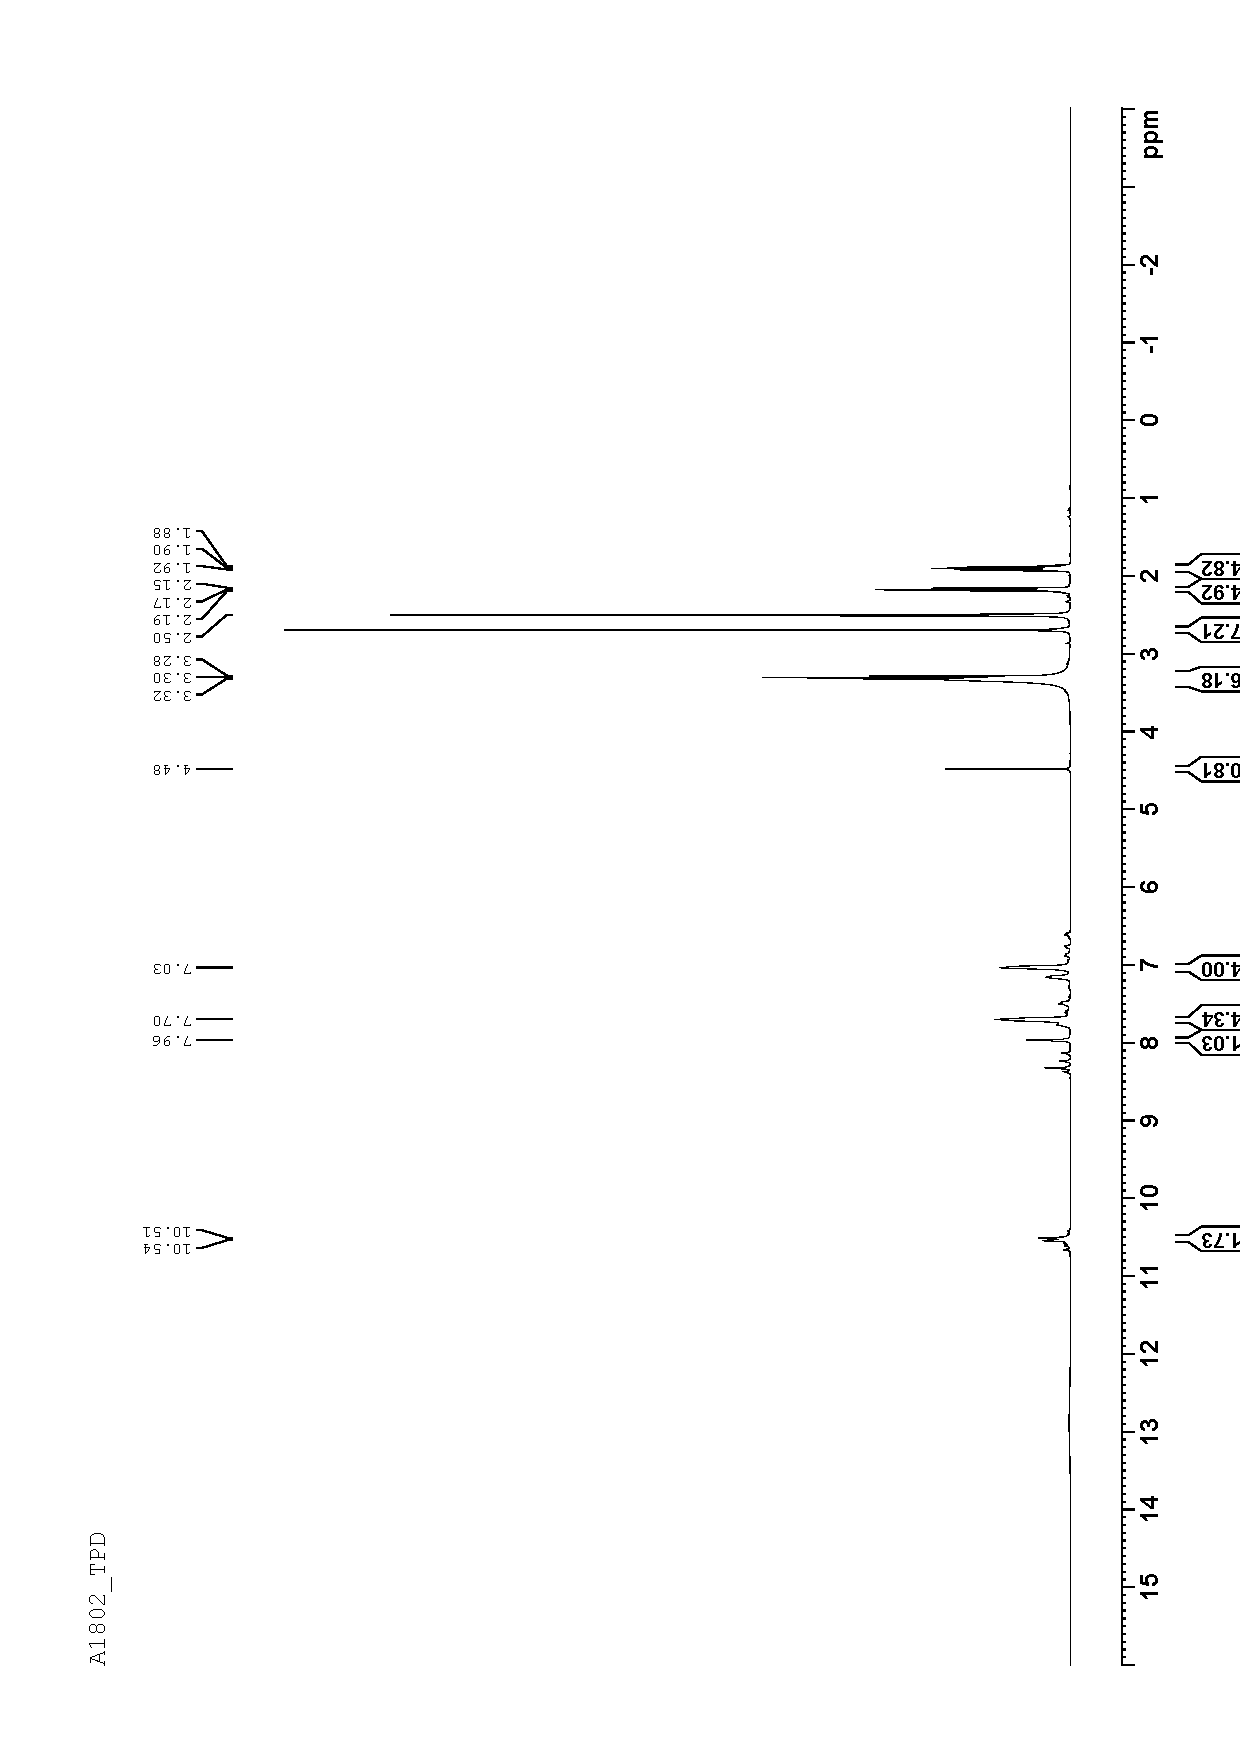
\includegraphics[angle=-90, width = \linewidth]{Images/A1802_finished.pdf}
    \caption{$^1$H NMR plot of attempted crosslinked sample with \ce{ZnCl2} and ethylene carbonate.}
\end{figure}

\begin{figure}
    \centering
    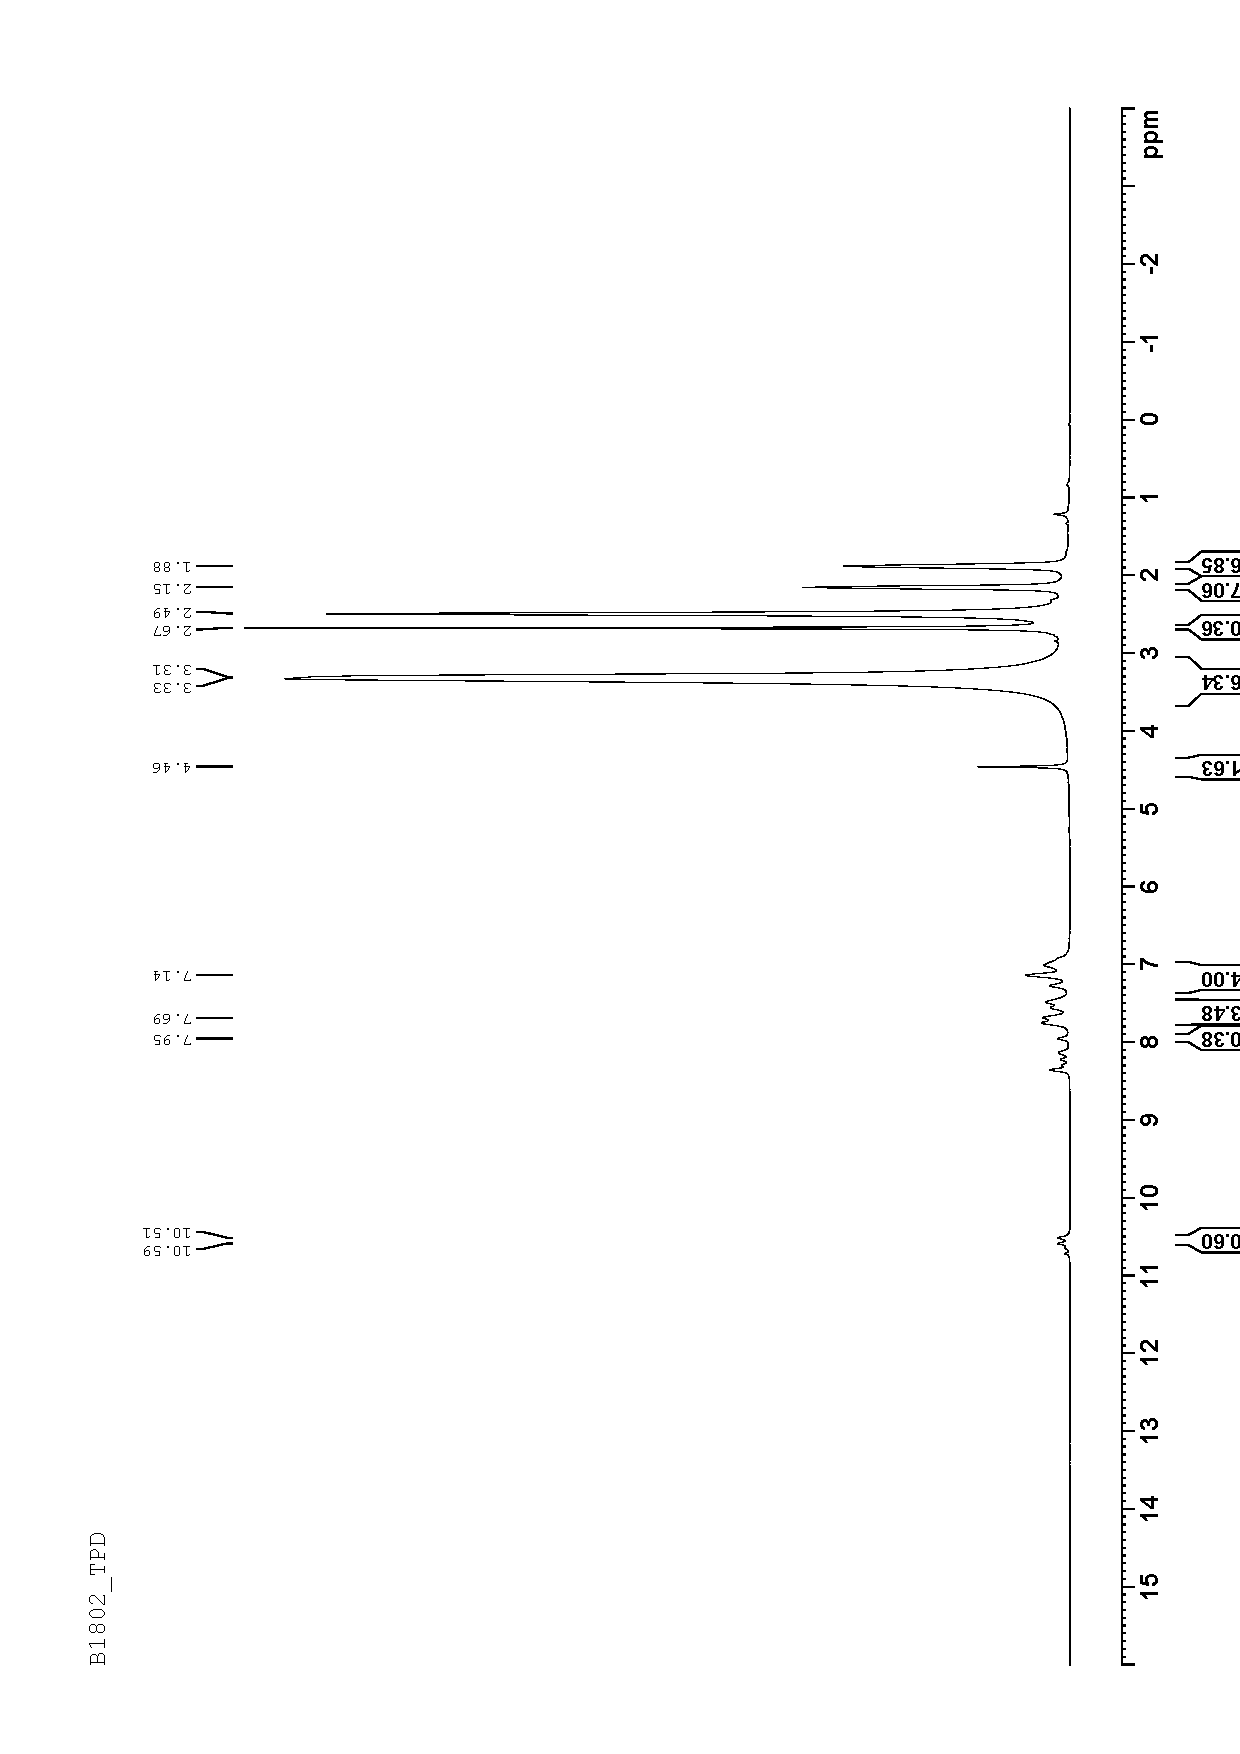
\includegraphics[angle=-90, width = \linewidth]{Images/B1802_finished.pdf}
     \caption{$^1$H NMR plot of attempted crosslinked sample with \ce{FeCl3} and ethylene carbonate.}
\end{figure}

\begin{figure}
    \centering
    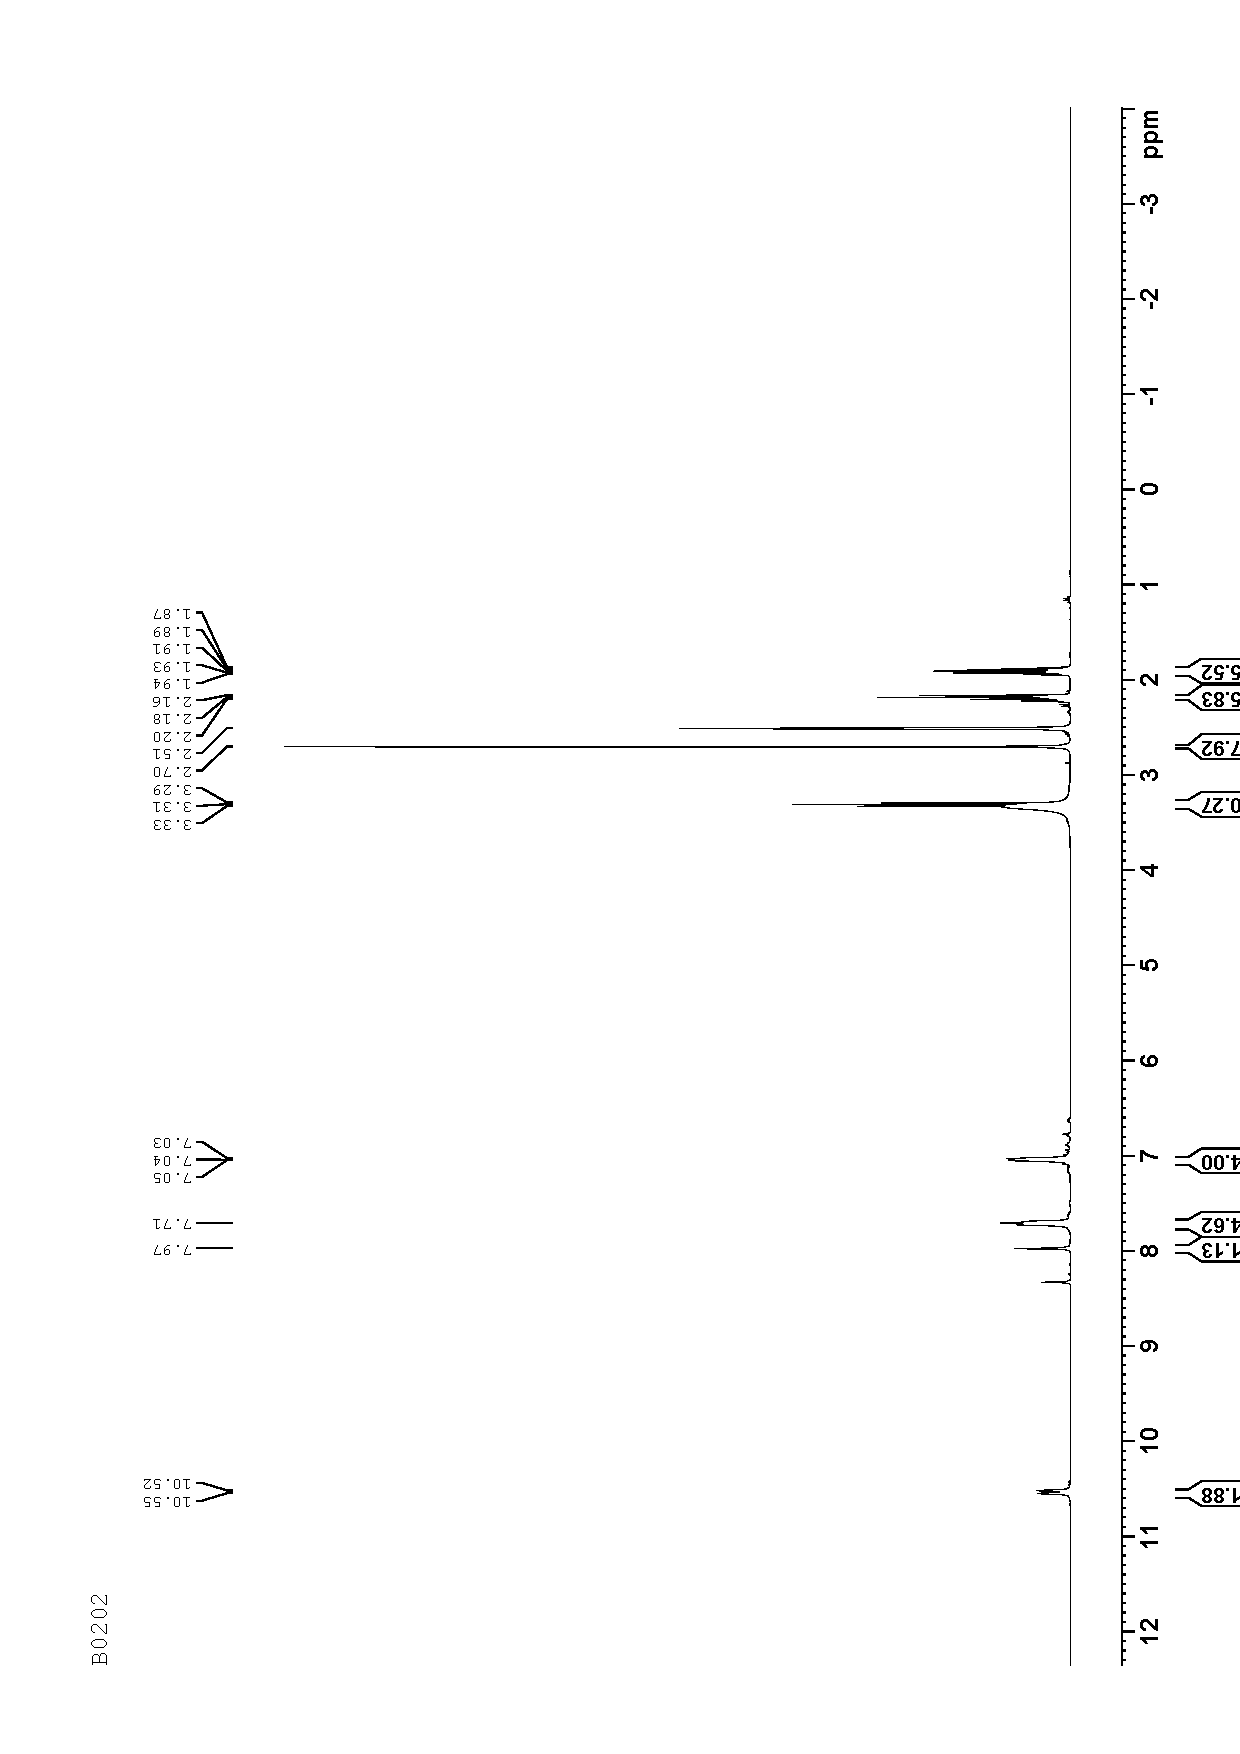
\includegraphics[angle=-90, width = \linewidth]{Images/B0202_finished.pdf}
    \caption{$^1$H NMR plot of polyamic acid}

\end{figure}

% \end{document}

\documentclass[12pt]{report}

% Preamble
\usepackage{graphicx}
\usepackage{setspace}
\usepackage[table,xcdraw]{xcolor}
\usepackage[a4paper, margin=1in]{geometry}
\usepackage{appendix}
\usepackage[superscript]{cite}
\usepackage{float}
\usepackage{listings}
\usepackage{color}
\usepackage{hyperref}
\usepackage{adjustbox}
\usepackage{caption}
\usepackage{setspace}
\usepackage{soul}
\usepackage{multirow}
\usepackage{tikz}
\usepackage{modiagram}
\usepackage{chemscheme}
\usepackage{chemfig}
\usepackage[version=4]{mhchem}
\usepackage{enumitem}
\usepackage{pdflscape}
\usepackage{amssymb}
\usepackage{gensymb}
\bibliographystyle{unsrt}

% Document setup
\setlength{\parindent}{0pt}
\setlength{\parskip}{1em}

% Code listing setup
\definecolor{dkgreen}{rgb}{0,0.6,0}
\definecolor{gray}{rgb}{0.5,0.5,0.5}
\definecolor{mauve}{rgb}{0.58,0,0.82}
\lstset{frame=tb,
  language=Python,
  aboveskip=3mm,
  belowskip=3mm,
  showstringspaces=false,
  columns=flexible,
  basicstyle=\ttfamily\small\setstretch{1},
  numbers=none,
  numberstyle=\tiny\color{gray},
  keywordstyle=\color{blue},
  commentstyle=\color{dkgreen},
  stringstyle=\color{mauve},
  breaklines=true,
  breakatwhitespace=true,
  tabsize=3
}

% Caption setup
\captionsetup{
  font={normal,stretch=1},
  justification=justified,
  singlelinecheck=false,
  aboveskip=8pt,
  belowskip=0pt,
  labelfont=bf
}

\begin{document}
\pagenumbering{roman}

% Create title page
\thispagestyle{empty}
\begin{center}
    
\includegraphics[width=7cm]{Images/University_of_Leeds_Logo.png}
\end{center}
\vspace{1cm}
 
\begin{center}
    \LARGE \textbf{Title}
    \LARGE \textbf{Subtitle}
\end{center}
\vspace{1cm}
% Author
\begin{center}
    \Large \textbf{Thomas P. Dean}
\end{center}
\vspace{3cm}

\begin{center}
    \Large \textbf{Masters Thesis}
\end{center}
\vspace{3cm}

% Facilty Info
\begin{center}
    \Large \textbf{The University of Leeds}

    \Large \textbf{Faculty of Engineering and Physical Sciences}
    
    \Large \textbf{School of Chemistry}
    
    \Large \textbf{School of Electronic and Electrical Engineering}
\end{center}
\vspace{1cm}
\begin{center}
    \Large \textbf{March 2026}
\end{center}

\normalsize
\doublespacing
\setcounter{page}{0}

\newpage
\thispagestyle{empty}
\vspace*{\fill} % Push the content to the vertical center
\begin{center}
\begin{quote}
\centering
    Acknowledgements.
\end{quote}
\end{center}
\vspace*{\fill} % Push the content to the vertical center

\newpage
\thispagestyle{empty}
\vspace*{\fill} % Push the content to the vertical center
\begin{center}
\begin{quote}
\centering
    Stick some more acknowledgments here.
\end{quote}
\end{center}
\vspace*{\fill} % Push the content to the vertical center
\newpage

\include{Abbreviations}

\chapter*{Abstract}

\chapter*{Acknowledgements}

Professor Bao N. Nguyen,
Professor James H. Chandler

Dr Ben, Dr Ben, Dr Josh, Dr Pete (STORM People)

Chem people

Sam Wilson, Alfred Alexander

Priestley + Porter techs

\chapter*{Intellectual Property}
The candidate confirms that the work submitted is his/her own and that appropriate credit has been given where reference has been made to the work of others.

This copy has been supplied on the understanding that it is copyright material and that no quotation from the thesis may be published without proper acknowledgment.

© 2026 The University of Leeds, Thomas P. Dean

\vspace{2cm}
%\makebox[6cm][c]{\raisebox{-2ex}{\includegraphics[width=6cm, height=2cm]{Images/Signiture.jpg}}}

\tableofcontents
\listoffigures
\listoftables

\newpage

\setcounter{page}{0}
\pagenumbering{arabic}


% ------------------------------------------------------------------------------
% Chapter 1
% Delete this content and replace with your own
%tis is a test sentence
% ------------------------------------------------------------------------------
\chapter{Introduction} % enter the name of the chapter here
\label{cha:introl} % enter the chapter label here (for cross referencing)

% \input{background}

\begin{figure}
    \centering
    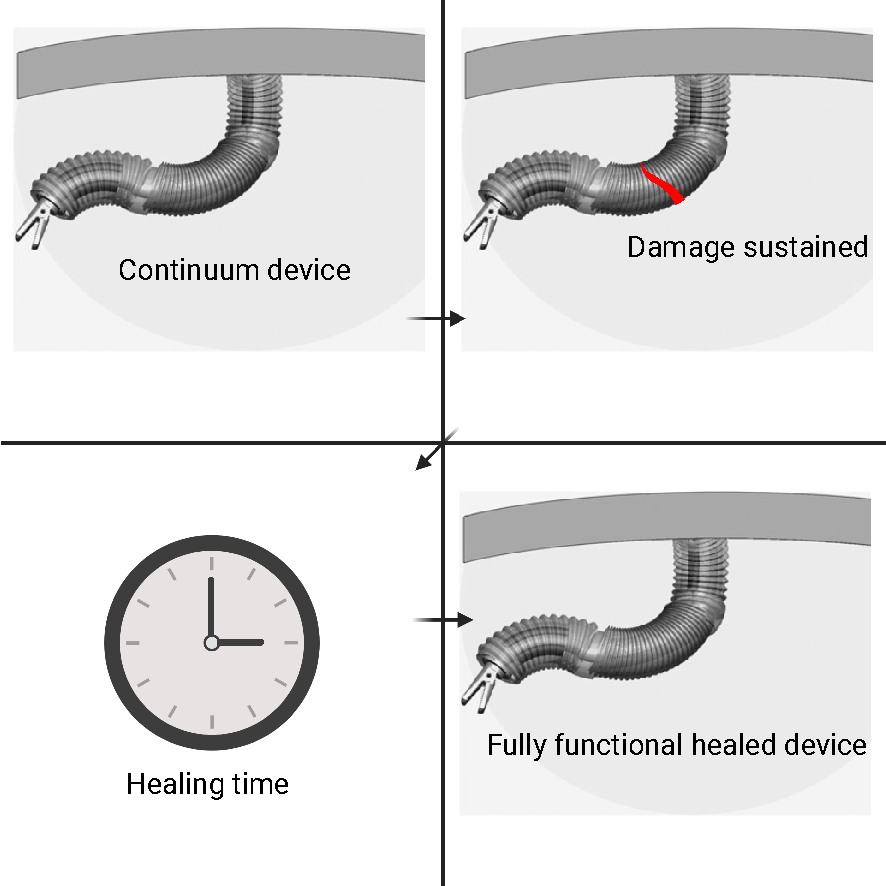
\includegraphics[width=0.8\linewidth]{Images/overview v3.pdf}
    \caption{A continuum device sustaining damage before self-healing and regaining full functionality using a modified image from \cite{cianchetti2014soft}}
    \label{fig:overview}
\end{figure}

\section{Importance and Applications of Soft Robotics}
Soft robots are devices known for their use of soft materials, compliant nature and near infinite degrees of freedom. Degrees of freedom (DOF) is a term related to the number of independent movements a robot can make in 3D space \cite{lynch2017modern}. Soft robots are usually nature inspired such as ``vine-like'' tip growing robots \cite{hawkes2017soft, davy2025magnetic}, ``snake like'' continuum robots \cite{anderson1967tenser, lloyd2020learnt} and ``hand-like'' soft grippers \cite{ilievski2011soft, guo2018soft}. The advantages of using a body that is highly deformable and with near-infinite DOF means these devices can be actively controlled to navigate tortuous environments with ease. 

This report focuses on continuum robots, often characterised by their long flexible bodies, commonly used for navigation and delivery or retrieval of objects in constrained environments \cite{russo2023continuum}. Continuum robots can be classified into ``continuous backbone'' and ``segmented back-bone'' designs \cite{russo2023continuum}. Continuous backbone devices are made from a soft and compliant material, in this report we will call these ``soft-bodied'', whereas, a segmented backbone refers to those that are made from hard, inflexible segments that are flexibly attached to achieve high curvatures, referred to here as ``hard-bodied''.

Hard-bodied continuum robots benefit from stiffer materials allowing a greater ease of control \cite{russo2023continuum} which can improve dexterity. However, they do not easily deform and are therefore more likely to impart a greater force on the surrounding environment \cite{davy2024vine}.  Hard continuum robots are often tendon driven, whereby the segments are joined by wires that can be pulled to give specific movements. Whereas soft bodied continuum robots can achieve high curvatures and low forces on surroundings \cite{rus2015design}, but are often harder to control due to their methods of actuation \cite{russo2023continuum} and can suffer from material failure \cite{abidi2017intrinsic}. Soft continuum robots commonly take the form of an inflated body, these can be controlled in many ways such as varying pressure \cite{hawkes2017soft}, strain limiting a specific region \cite{guo2024encoded, dean2025anisotropic} or magnetic actuation \cite{davy2025magnetic, davy2024vine}. Pressurised systems that rely on fluids need a constant seal to maintain function as opposed to a segmented tendon driven approach that can be partially damaged and remain actuatable. This motivates the utilisation of resilient materials, such as self-healing polymers, for soft robotic contexts.



\section{Types of Self-Healing Polymers}

\begin{figure}
    \centering
    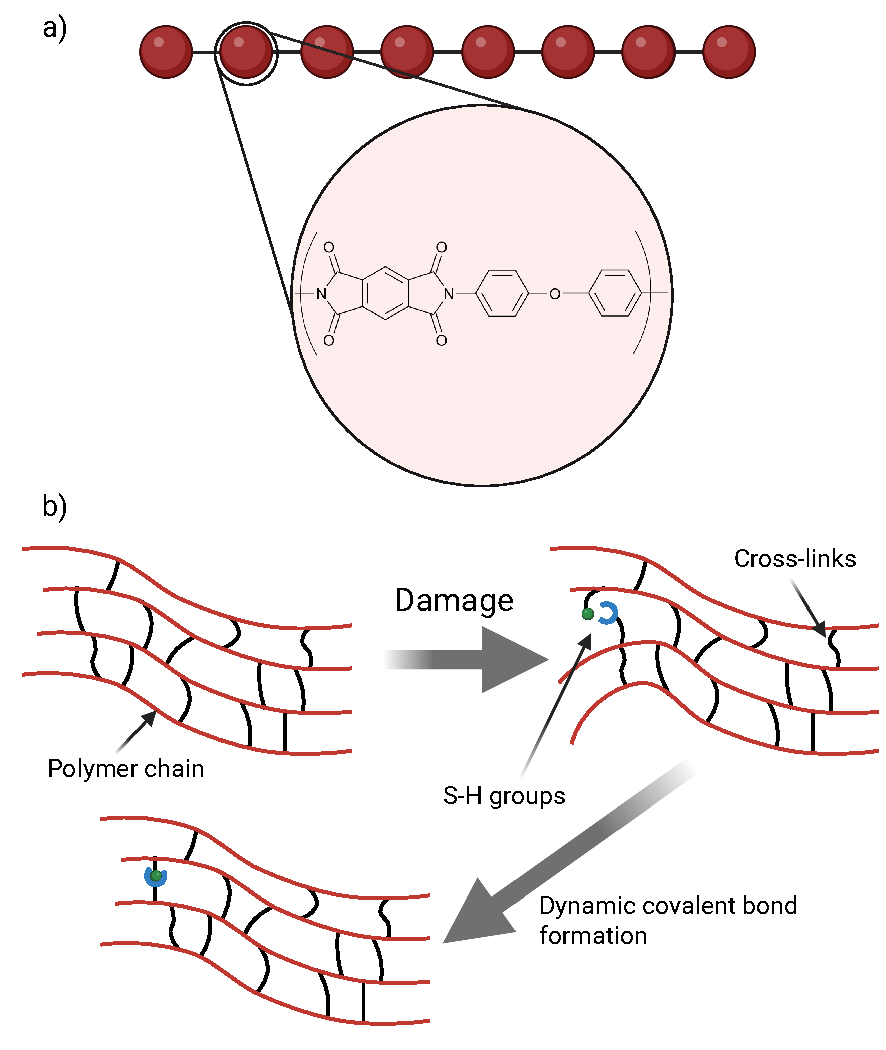
\includegraphics[width=1\linewidth]{Images/Self healing polymer.pdf}
    \caption{a) The polymer chain with a repeating chemical sub-unit. b) The mechanism of damage and repair for a self-healing polymer}
    \label{fig:shpolymer}
\end{figure}

Polymers are a type of molecule that consists of several repeating sub-units, these form chains that are combined many times over to form materials. Self-healing (S-H) polymers are a type of polymer that can heal damage \cite{srivastav2025comprehensive}. This occurs through reactions and interactions between multiple polymer chains to reconnect chains that have been shifted apart through damage. The process of damaging or cutting a polymer does not break bonds in the polymer backbone but instead can break interchain interactions called cross-linking, allowing the chains to drift apart, reforming the cross-linking interactions will ``heal" the material \cite{binder2013self}. 

S-H polymers can be classified into intrinsic or extrinsic healing, and autonomous or non-autonomous \cite{terryn2021review}. Materials with an intrinsic healing capacity involve a healing mechanism through chemical bonds or interactions that are continuously present in the polymer, rather than extrinsic healing, such as capsules of ``healing" material that are broken through damage and causing the material to reform \cite{white2001autonomic}. Autonomy refers to the healing process occurring without external input. For example, capsules that burst upon damage of the material and release a healing agent are classified as autonomous, whereas a photochemical reaction that needs UV light to activate \cite{trenor2004coumarins,froimowicz2011photoreactive} is a non-autonomous mechanism. 


\section{Comparison of Different Self-Healing Pathways}
There are a variety of different pathways that can be taken to create a S-H polymer depending on the chemistry of the initial polymer. The pathways that will be focused on are intrinsically self-healed types, however, both autonomous and non-autonomous types will be considered.

The three pathways below rely on a property of some electrons called conjugation. Conjugation occurs when specific electron orbitals overlap in such as way that allows the electrons to move around the molecule. This is often exploited with a property of some atoms called electronegativity, having a highly electronegative atom in a molecule will attract conjugated electrons to create a local high density region of electrons and therefore a polarisation in a molecule. 

Dynamic covalent bonds can form and break based on the conditions applied to them \cite{guo2025diels} and they are ideal for use as mechanisms for S-H due to their intrinsic nature and reliability in production of high yields \cite{nicolaou2002diels}. This report investigates the use of two types of dynamic covalent bonding, Diels-Alder and Michael additions, and an example of a supramolecular interaction. Supramolecular chemistry is based on interactions that are non-covalent and may be more suited to a soft material \cite{yang2018self}. This is due to the self-healing mechanism of the cross-links that forms interactions therefore the polymer chains can move semi-independently \cite{wanasinghe2022dynamic,yang2018self}. Whereas, a dynamic covalent bond has a much higher bond energy \cite{guo2025diels} and can therefore get closer to the original physical properties of a polymer.

\subsection{Using a Diels-Alder Addition as a Self-Healing Pathway}

\begin{figure}
    \centering
    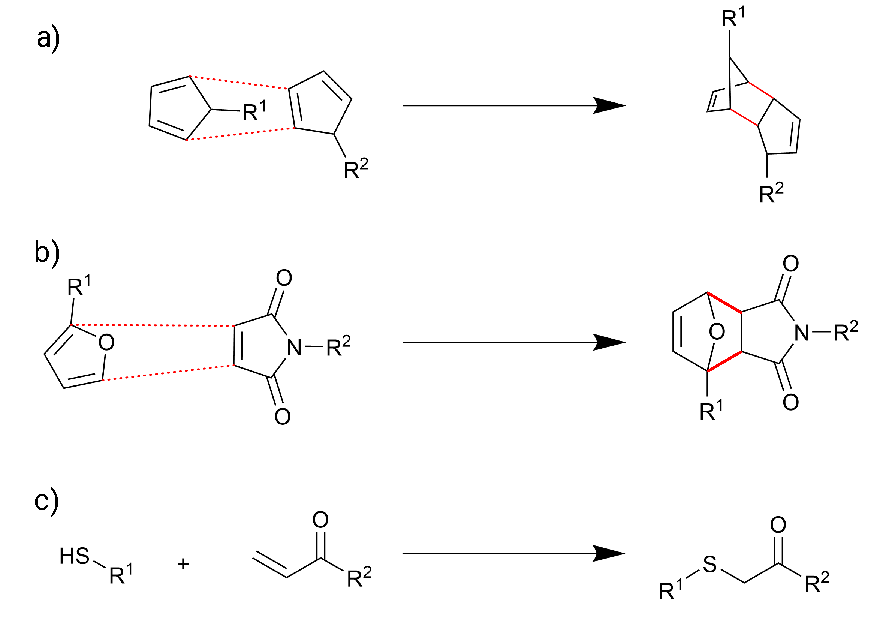
\includegraphics[width=0.8\linewidth]{Images/DA reactions.pdf}
    \caption{a) A Diels-Alder reaction between two molecules of cylopentadiene. b) A Diels-Alder reaction between a furan and maleimide. c) A Thiol-Michael Addition between a thiol and a conjugated alkene. }
    \label{fig:dareactions}
\end{figure}
Diels-Alder (DA) reactions require a diene, a class of molecule characterised by having two sets of double bonds, and an alkene (``dieneophile") \cite{ratwani2023self,guo2025diels}. The reaction occurs when conjugated electrons from the diene are free to move to form new bonds with the carbons either side of the alkene double bond, this creates a new ring structure. A faster reaction is generally observed with an electron rich diene and an electron poor dienophile \cite{briou2021trends}. The electronic character of the reagents can be altered by changing their local substituents. This class of reactions can have lots of different conditions depending on the molecules involved. Some variations can occur at room temperature \cite{huertas2009solvent}, which may make them an ideal choice for an autonomously healed medical device as the healing can occur whilst deployed in the body. However, many DA reactions are light \cite{trenor2004coumarins,froimowicz2011photoreactive} or heat activated \cite{li2014situ}.

Some molecules such as cyclopentadiene can perform a DA reaction with itself, this has the potential to be an ideal choice for a S-H polymer as the molecule will never be in close proximity to a molecule that it cannot react with. However, some evidence has shown that the bonds formed are not very strong and therefore high tensile strength materials may not be possible \cite{ratwani2023self}.

One of the most common types of DA reaction is a heat activated reaction between a derivative of both furan and maleimide \cite{ingoglia2014microencapsulation}. They react extremely accurately and require mild conditions \cite{ratwani2023self}, therefore they are very suitable for application as a robotics material.
One of the reasons that this reaction is so effective is that the maleimide has electron withdrawing carbonyl groups which make the dieneophile electron poor and therefore reacting faster. However, this mechanism has a disadvantage compared to cyclopentadiene as there are two halves of the end product. Therefore, there must be two different processes occurring to create both the furan substituted and maleimide substituted chains. This increases the number of total steps in the reaction which increases the risk of low reaction yields and wasted material. 


\subsection{Using a Thiol-Michael Addition as a Self-Healing Pathway}
Thiol Michael additions are a type of reaction that relies on a thiol, a molecule characterised by a sulfur containing group and a conjugated alkene \cite{nair2014thiol}. The conjugated alkene used in a Michael addition is with a carbonyl group that will attract the electrons from the alkene to allow the thiol group to react. This has a similar advantage to the Diels-Alder reaction that it is not totally dependant on specific reactants merely groups of reactants. Therefore slight changes can be made to the adjoining groups to tweak the reaction conditions. This has been previously shown to have been successful with a heat activated reaction that could heal scratches after 15 to 30 minutes at 60 \degree C \cite{kuhl2016self}. 

\subsection{Using a Pi-Stacking Approach as a Self-Healing Pathway}
Pi-Stacking is a type of intermolecular interaction whereby conjugated systems interact based on the neighbouring substituents determining if a region is electron rich or poor. These electron disparities cause an electrostatic interaction. This method commonly uses pyrenyl groups, these are polycyclic aromatic compounds, a very pi-electron rich species. These can be interacted with a napthalene diimide complex, an electron poor pi-system to give four pi-stacking interactions. A method has shown the creation of a polymer chain end group which can sandwich a napthalene group within two pyrenyl groups. \cite{burattini2011supramolecular}. This method can be combined with other intermolecular interactions like hydrogen bonding \cite{yuan2025self} or mettalosupramolecular interactions to give a stronger interaction \cite{mei2016highly}.


\section{Applications of Self-Healing Polymers in Soft Robotics}

Continuing the theme of biological inspiration of soft robotics, S-H polymers can be used to extend the lifespan of components. In soft continuum robots, the goal is usually to make the robot softer than the environment surrounding it \cite{rus2015design}. This presents challenges in abrasive environments that can damage the device. It is therefore evident that a damage resilient material would be useful. Damage resilient materials can take multiple forms: Damage isolation, material elasticity, physical self healing such as low melting temperature materials and chemical self healing \cite{bilodeau2017self}.



\subsection{State of the Art Self-Healing Soft Robots}
 State-of-the-art approaches using intrinsic S-H mechanisms are commonly based on DA chemistry \cite{terryn2021review}. These have been successfully implemented in tendon-driven \cite{roels2019multi} and pneumatically controlled soft robotic devices \cite{terryn2020room, terryn2017pneumatic}. Such devices are capable of recovering from macroscopic damage, including punctures and cuts. Additionally, there are non-covalent approaches that utilize hydrogen bonding in the development of soft self-healing actuators, such as in McKibben muscle designs \cite{lopez2020autonomous}.

\subsection{Requirements for Self-Healing Polymers in Soft Robotics}
Terryn \textit{et al.} \cite{terryn2021review} states that there are 5 main criteria for a S-H polymer; macroscopic damage must be healed completely; healing can take place multiple times at the same location; there are minimal material property changes after healing; elastomeric behaviour is achieved; the reprocessing and recycling of a material is possible. Here we propose that elastomeric behaviours are non-essential and a more useful requirement would involve a timely S-H reaction.  


\section{Limitations with Current Materials for Soft Robotics}

Damage control whilst a device is active can be a challenge \cite{kashef2025toward}, this shows a need for autonomous S-H \cite{terryn2021review}. Non-autonomous S-H can be made ``functionally autonomous" through the use of stimuli responsive mechanisms, however, the current options are slow in operation \cite{kashef2025toward}. Currently recovery timescales of applied S-H polymers are around 25 hours \cite{terryn2017pneumatic, bilodeau2017self}. By altering the polymer used or S-H pathway this could be improved. There is also a lack of an easy synthesis route for many of the current polymer options \cite{bilodeau2017self}, thereby increasing the cost and reducing widespread use. Also the number of damage-repair cycles in these devices are low, such as 3 or less \cite{terryn2017pneumatic}. Most devices do not achieve all five criteria laid out in the Terryn \textit{et al.} review \cite{terryn2021review}, such as the McKibben design of A. Lopez Diaz \textit{et al.} \cite{lopez2020autonomous} only reporting a healing efficiency of 65\%.

% ------------------------------------------------------------------------------
% Chapter 2
% ------------------------------------------------------------------------------
\chapter{Project Aims and Objectives} % enter the name of the chapter here
\label{cha:aims} % enter the chapter label here (for cross referencing)

% \input{aims}



\section{Aims and Objectives of this Project}
The aim of this project is to understand the use of a self-healing polyimide in a soft robotics context.

We hypothesise that the incorporation of a S-H polyimide into soft robotic components will enhance their lifespan.


The objectives of this project are to:
\begin{itemize}
    \item Investigate the alteration of a polyimide through a Diels-Alder pathway to achieve a self-healing polymer 
    \item Investigate the processability of the modified polymer through material tests such as melting point analysis. 
    \item Based on the processability, apply the polymer to either a sheet film material or a moulded component suitable for use as a soft robotics component
    \item Based upon the form of the modified polymer construct and use as an inflatable soft continuum robot or for use in other hard or soft bodied components 
    \item Test component/robot through different techniques such as tensile testing and force characterisation.
    \item If time allows, design and construct a system that can autonomously self heal components. For example, using a UV controlled self healing reaction, the flow rate of air into an inflatable device could be measured so that if the flow changed a UV light could be activated thereby autonomously self-healing the components.
\end{itemize}






 
\chapter{Towards the Synthesis of a Self-Healing Polymer} % enter the name of the chapter here
\label{cha:chem} % enter the chapter label here (for cross referencing)

This study aims to lay initial ground-work for the development of a self-healing polymer. This involves Kapton\textsuperscript{\textregistered}, a commercially available polyimide, well known for highly resilient properties. This section covers the initial process for the alteration of polyimide via hydrolysis in order to expose reactive carboxylic acid (COOH) groups and the subsequent reactions with these exposed COOH groups. Hydrolysis is a process in which polyimide is broken down into a precursor, polyamic acid, this exposes regions in which additional reactivity can be added. One route to the development of a self healing polymer is through the formation of crosslinks at these exposed COOH sites. Specific types of crosslinks can dynamically break and reform to achieve a material that can repair itself. A proof of concept reaction between polyamic acid and ethylene carbonate, a crosslinking reagent, was attempted as a preliminary demonstration.


\section{Results}
\subsection{Hydrolysis of the Polyimide}
The hydrolysis of the polyimide follows a standard mechanism for hydrolysis of an amide to a carboxylic acid using sodium hydroxide (NaOH). These show the hydroxy group attacking the carbonyl which then breaks the C-N bond and gives the carboxylic acid free.

During the formation of the hydrolysed version, the polymer sheets were converted into a light orange suspension which was filtered to give a pale orange precipitate.

\subsubsection{Structural Analysis}
Structural determination was conducted via Infrared spectroscopy. A comparison was made between the attempted hydrolysis of the sheets and a purchased form (polyamic acid). 

\subsection{Cross-linking of the Polyimide}
Cross-linking attempts follow a mechanism as proposed by ( put reference here), where ethylene carbonate is used to form an ester with the carboxylic acids on neighbouring polymer chains, thereby joining them together with a "cross-link". This was performed with three different salts ( TEAB, $ZnCl_2$, $FeCl_3$) as catalysts. 

During the cross-linking reaction with TEAB, an orange-brown suspension was formed that when washed, filtered and freeze dried gave a pale orange powder. With $ZnCl_2$, the liquid was a dark orange clear liquid that, when water was added, gave a single clump of grey polymeric residue. This was freeze dried to remove the excess water and then analysed. The cross-linking reaction with the $FeCl_3$, gave a dark orange/brown gel, which gave a grey gum-like texture in small pieces when water was added. This was also frozen and analysed. 

\subsubsection{Infrared Spectrum analysis}



% \section{Hydrolysis of a Polyimide}
% The hydrolysis of the poylimide (kapton) is needed to open an amide bond on the imide ring to reveal a carrboxylic acid group whilst the bolymer back bone is still intact. This will make the polymer soluble, however since the polymer is insoluble currently the only attack will be on the polymer surface. This was completed with sodium hydroxide in (solvent) and in the monowave reactor for (x time)

% The structure of the proposed polyimide is shown in figure (x). This structure has multiple imide rings that we hypothesise are a good starting point for introducing reactivity. 

% The partial hydrolysis of these rings was performed with Sodium hydroxide solution (in dmso). This reaction was performed in the monowave reactor. The monowave reactor is a reaction vessel that is within a machine that can reduce the pressure on the environment. This is useful as the boiling point of the solvent is increase with lower pressure. Therefore a reaction that can only be performed above a certain temperature like this one can be done in solvent with a lower boiling point than the reactuion requirements.

% \subsection{}


% %input graph about changinh boiling point of solvent with pressure

% \subsection{Comparison of Hydrolysed Polyimide versus Purchased Polyamic Acid}
% the hydrolysed polyimide should have a similar ir as a purchased form of the polyimide as both have a exposed carboxylic acid group, therefore there will be a characteristic shift at (wavenumber).


% \subsection{Spectral Analysis}
% Structural determination was performed with infrared (IR) spectroscopy and Ultraviolet - visible (UV-Vis) spectroscopy. Key IR peaks for the unmodified Kapton are (x), the key peask for the modified kapton are (x) and the key peaks for the purchased Polyamic acid are (y). 



% \section{Crosslinking of Polyamic Acid}

% crosslinking of polyamic acid was done in a reaction with the ethylene carbonate and an ammonium bromide salt this gave the reaction as in a similar process as in (this paper ). the carboxylic acid groups react with the ethylene carbonate to form either an ester with a hydroxy after an alkyl chain on one of the polymer chains or it will like the polymer chains together by forming a diester. 


% Using the monowave uses a 10mL reaction tube that was filled with 4ml of reagents to leave room for the co2 that is released in the reaction. The volume of co2 released was calculated using
% $PV = nRT$ which was rearranged to $n = \frac{PV}{RT}$. The monowave 50 has a maximum pressure of 20 bar, so we opted for a maximum of 5 bar for safety. this was combined with a temperature of 150$\degree$C to give: 

% \[n = \frac{PV}{RT}\]
% \[n = \]


% THis was the total number of co2 mo

% \section{Addition of Diels-Alder Groups}

% \section{Experimental}
% Kapton (poly-oxydiphenylene-pyromellitimide) sheets were cut into small pieces ($\approx$ 2mm$^2$). These were added to a solution of NaOH (vol and mol here) and heated to 120 $\degree$C in a monowave reactor set to ramp for 20 mins and hold for 20 and 40 mins successively. The reaction gave no observable difference in the Kapton sheet

\section{Experimental}
\subsection{The Hydrolysis of a Polyimide}
Poly..... (Kapton) film (0.2g, thickness of x) was cut into pieces of approx. 3mm$^2$, these were mixed with a solution of NaOH () in a reaction tube. This tube was placed into a monowave reactor that was set to ramp for 20 minutes and hold for 20 minutes at 100 $\degree$C. A sample was taken and the remaining mixture was reacted again on the monowave for ramp 20 mins and hold 20 minutes at 100$\degree$C. There was no observable difference in the Kapton film. Then this was thoroughly washed with water and IR was collected.

\subsection{Cross-linking with TEAB and Ethylene carbonate}
A mixture of polyamic acid (0.51mL, conc) was mixed with ethylene carbonate () and tetraethylammonium bromide (). This was mixed in a monowave reactor set to ramp for 20 minutes and hold for 1 hour at 150 $\degree$C. This gave an orange suspension that was dried to give a pale orange powder as the final product (grams, yield).
IR (solid): 

\subsection{Cross-linking with $ZnCl_2$ and Ethylene carbonate}
A mixture of polyamic acid (0.51mL, conc) was mixed with ethylene carbonate () and Zinc chloride (). This was mixed in a monowave reactor set to ramp for 20 minutes and hold for 1 hour at 100 $\degree$C. This gave dark orange clear liquid that was dried to give a () as the final product (grams, yield).
IR (solid): 

\subsection{Cross-linking with $FeCl_3$ and Ethylene carbonate}
A mixture of polyamic acid (0.51mL, conc) was mixed with ethylene carbonate () and Iron(III) chloride (). This was mixed in a monowave reactor set to ramp for 20 minutes and hold for 1 hour at 100 $\degree$C. This gave a dark orange clear gel that was dried to give a () as the final product (grams, yield).
IR (solid): 
%%ethics
\chapter{Construction of a Bellows Based Actuator} % enter the name of the chapter here
\label{cha:storm} % enter the chapter label here (for cross referencing)

In this chapter, the focus shifts towards robotics. Here a device is constructed where the majority of the outer surface is constructed from the same polyimide in which chemiocal modification was previously attempted. The focus of this aims to make use of the highly resilient properties that are already present within the polyimide material and show the capabilities of a device constructed with them. 

This chapter covers the design and construction of a continuum robot with a protective outer layer constructed from folded polyimide sheets. This protective layer is tested for temperature stability. The manouverabiliy of this device is also tested in 3D space before demonstrating this in an arbitrary setting and a medical setting, a space that soft-robotics are currently revolutionising. 

a space that requires material resilience.


 \section{Design}
Actuators were constructed using a combination of a folded polyimide sleeve and a internal  multilumen silicon tube with nitinol wires for actuation. Our methodology is inspired by similar "bellows-style" approaches to construct continuum devices (references) with the key difference in the use of Polyimide sheets (Kapton) forming the main body of the device.

This work focuses on the use of Kapton (thickness = ) due to its good robustness and high temperature capabilities.

\subsection{Construction of a Folded Protective Sleeve}
The polyimide film was folded into a []-style design as based on the previously published work [reference]. To achieve the folding a 2D drawing of the fold lines was drawn in Fusion360 and printed onto paper. This paper was taped to the table and a sheet of Kapton was taped over the top, the Kapton is clear so the printed lines are visible through. The lines were then traced onto the Kapton with a ruler and a ballpoint pen. The ballpoint pen marked the desired fold lines and also partially indented on the lines. The sheet of kapton was removed from the table and the outer edge was cut with scissors. The Kapton sheet was then folded along the lines as shown in the figure [ref figure]. The folds on the sheet were puished back out and the kapton was rolled into a cylinder. This was taped along the overlapped edge to form a temporary seal while maintaining care to line up the folds. The tape was removed in small sections and JBweld HighHeat was applied until the whole adhesion region. This was threaded onto a plastic tube with a diameter approx. 2mm smaller than the kapton sleeve. The sleeve was taped to the tube and the adhesion region was taped over the top to clamp the glued region. This was left for 24 hours to cure. The glueing and the curing process was performed in a Fume cupboard [brand/details] due to the risk of respiratory irritation through the curing process. After curing, a strip of Kapton tape was placed over the edge on the adhesion region. This improved the flexiblity of the region. 


For the proposed design, the film selected was Kapton\textsuperscript{\textregistered} ( Supplier, thickness). 

\subsubsection{Manual folding versus using a plotter}
A commercially available plotter (Cricut\textsuperscript{\textregistered}) was used with a scribe tool and a cutter to achieve a rapid manufacturing of a folded sleeve. This was attempted with paper initally for cheap prototyping and then transferring to the polymer film. 

The paper was easy however the polyimide did not take up the scores so easily. We demonstrated this difference by using the plotter to score a 5cm line on piece of 80gsm paper (roughly 0.25mm) and two pieces of Kapton (thicknesses). These were attached to the jaws of a vice and compressed to form a crease on the scored line. On the paper attempt, after the material was allowed to relax, a defined crease was left in the material. In comparison, the Kapton did not take up the crease and when relaxed, remianed in a curve.

\subsection{Complete Assembly}
The complete assembly was formed with the polyimide sleeve, the silicon continuum device and 3D printed parts. The construction method is as follows: a sheet of polyimide is marked with the desired folding pattern (as shown in figure), the sheet is folded by hand before being shaped into a tube and glued along an overlapping edge. The folds are encouraged into place and one end is sealed. This is the assembled with 3D printed parts to form the actuator.

The silicon actuator contains 7 holes where three lengths of nitinol wire were threaded through and fastened with two grub screws each in 3D printed handles. This leaves a separate tube through the centre of the silicon tube that can be used for targeted delivery of liquid or components such as naneye cameras for observation.


 \section{Results}

\subsection{Stiffness Characterisation}

\subsection{Workspace Characterisation}
 \section{Methodology}

Our methodology is inspired by similar "bellows-style" approaches to construct continuum devices (references) with the  key difference in the use of Polyimide sheets (Kapton) forming the main body of the device.



This work focuses on the use of Kapton (thickness = ) due to its good robustness and high temperature capabilities.

\subsection{Stiffness Characterisation}

\subsection{Temperature Stability of the Bellows}

\subsection{Workspace Characterisation}


 


\bibliography{references}

% \begin{appendices}
%     % \include{work}
    
% \end{appendices}

\end{document}